\chapter{Лекция}
\label{ch:intro}

\section*{\textbf{Введение}}

На прошлом занятии мы работали с Adalm Pluto напрямую из C++, приняли семплы и записали их в файл. На этом занятии чуть более подробно углубимся в этот процесс и попробуем
сформировать свои собственные семплы и отправим их с SDR.

\section*{\textbf{Структура семплов в Pluto SDR}}

\begin{figure}[H]
    \centering
    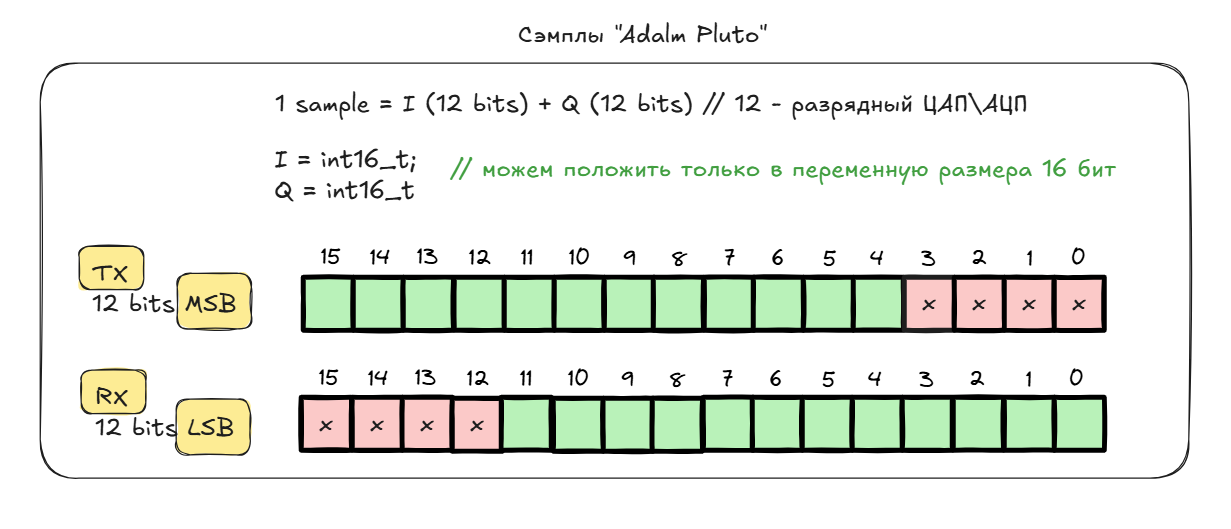
\includegraphics[width=1.0\textwidth]{sample_struct.png}
    \caption{Структура семплов}
\end{figure}

Pluto SDR имеет 12-ти битный АЦП, это значит, что для I и Q максимальное значение составляет $2^12 = 4096$, но один бит займет знак, поэтому I и Q будут принимать значения
из отреза [-2048;2047]. Для хранения I или Q в С++ используется тип данных int16\_t (если брать меньше, то семпл не поместится). Таким образом один семпл занимает 4 байта
памяти. Также есть вариант хранить семплы в одной переменной int32\_t, но в таком случае для получения доступа к I или Q придется использовать битовые сдвиги или накладывать
маски. \\

Стоит отметить, что Pluto SDR странно работает с TX семплами (которые хотим передавать) и интерпритирует как семплы последние 12 бит переменной (если начинать отсчет от
младшего бита), поэтому необходимо сдвигать значение I и Q на 4 бита влево (<<4) при работе с tx буффером, чтобы Pluto SDR корректно их интерпритировал. 

\section*{\textbf{Структура буффера семплов в Pluto SDR}}

\begin{figure}[H]
    \centering
    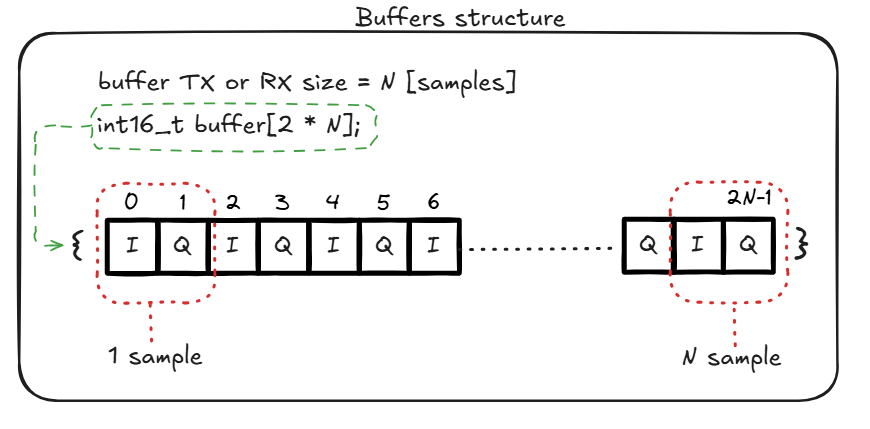
\includegraphics[width=1.0\textwidth]{buffer_struct.png}
    \caption{Структура буффера}
\end{figure}

Семпл состоит из компонент I и Q, которые хранятся последовательно друг за другом, т.е в буффере будет иметь последовательность вида $I_0, Q_0, I_1, Q_1, ... , I_n, Q_n$, поэтому
если мы хотим принять/передать N семплов, то буффер должен быть размером 2N, т.к семпл состоит из двух чисел.

\section*{\textbf{Запись RX семплов в буффер в Pluto SDR}}

\begin{figure}[H]
    \centering
    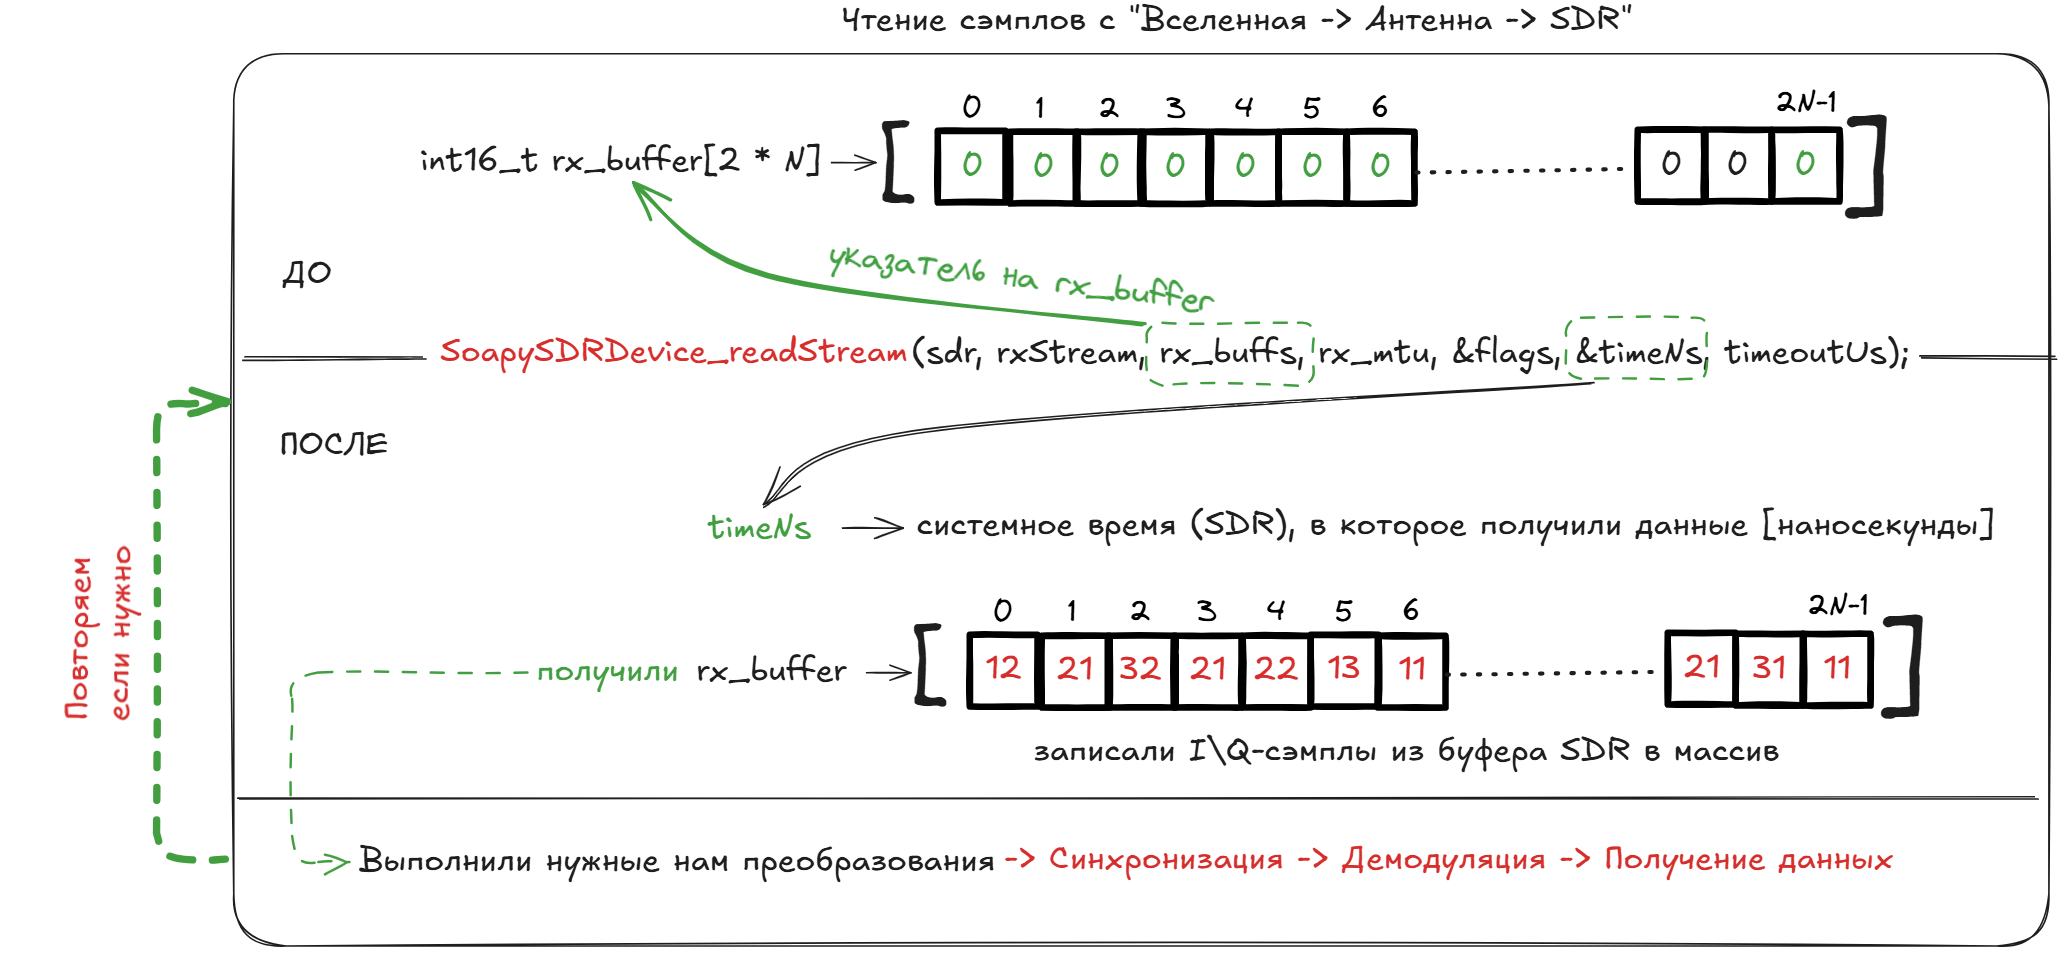
\includegraphics[width=1.0\textwidth]{sample_read.png}
    \caption{Запись RX семплов}
\end{figure}

Для записи RX семплов в буффер используется функция SoapySDRDevice\_readStream(), в которую необходимо перредать указатель на буффер, в который хотим писать, и кол-во 
семплов, которые мы хотим записать, и еще некоторые дополнительные параметры. После выполнение функции в наш буффер будут записаны семплы, принятые SDR.

\section*{\textbf{Создание своих семплов и их отправка в Pluto SDR}}

\begin{figure}[H]
    \centering
    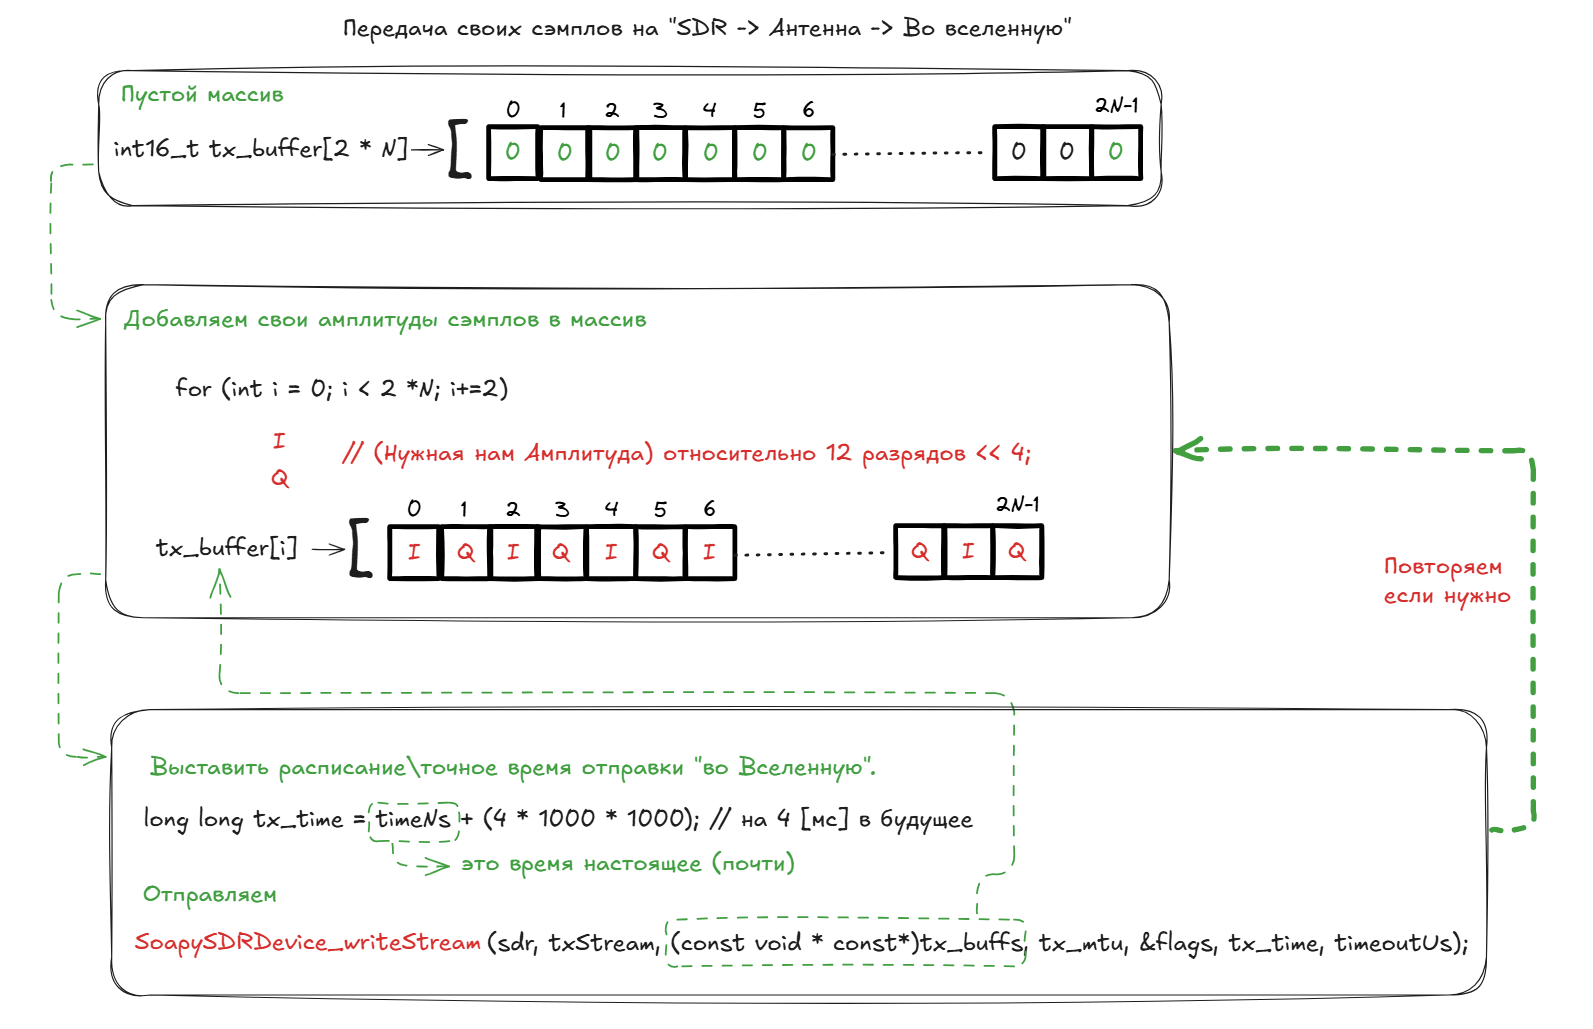
\includegraphics[width=1.0\textwidth]{sample_tx.png}
    \caption{Создание и отправка семплов}
\end{figure}

Для отправки семплов сначала необходимо заполнить tx буффер самими семплами. Формировать сами I и Q можно разными способами, но самое главное разместить их в правильном порядке.
Для самой отправки используется функция SoapySDRDevice\_writeStream(), в которую необходимо передать указатель на буффер с семплами и время, через которое семплы будут
отправлены, а также дополнительные параметры. После вызова функции через 4нс наши семплы отправятся с Pluto SDR.


\endinput

